%
% tp 2 mna
% 

% Use emulateapj instead to make Apj format.
% YOU SHOULD REMOVE THE TABLE OF
% CONTENTS PAGE WHEN USING APJ FORMAT.
\documentclass[11pt,a4paper]{emulateapj}
\bibliographystyle{apj}


%define general packages
\usepackage{epsfig}
\usepackage{amsmath}
\usepackage{natbib}

% spanish packages
\usepackage[utf8]{inputenc}
\usepackage[spanish]{babel}
\languageshorthands{none}
\noextrasspanish
\let\layoutspanish\relax
\usepackage[spanish]{babel}
\renewcommand\shorthandsspanish{}

%internal short cuts
\def \HgA {H$\gamma_A$}
\def \gon {Gonz\'{a}lez}
\def \Hbp {H$\beta ^\prime$}
\def \warn {{\sffamily\bfseries\large WARNING, ARREGLAR:}}









\begin{document}

\submitted{Departamento Ing. en Informática, ITBA}
\title{Filtros espaciales en imagenes mediante el paso del dominio de los colores al dominio de las frecuencias}
\author{Williams M. \& Aráoz M.}
\date{\today}


\begin{abstract}
\warn{hacer abstract}
\end{abstract}

\maketitle




\section{Introduccción}
\label{sec:introduccion}

%\begin{figure*}
%  \begin{center}
%    \leavevmode
%      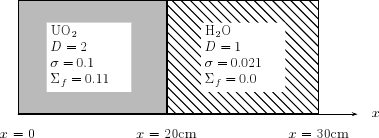
\psfig{file=images/img1.png, width=254px}
%       \caption[Esquema simple del reactor]{Modelo de un ractor nuclear unidimensional.
%         Diagrama adaptado de \citet{diaz10}.}
%     \label{fig:esquema}
%  \end{center}
%\end{figure*}


\section{Seccion 2}
\label{sec:sec2}

\section{Seccion 3}
\label{sec:sec3}




\section{Resultados y Conclusiones}
\label{sec:resultadosyconclusiones}

%
\bibliography{paper}

\end{document}

